\begin{frame}[hoved]
	\frametitle{Implementation}
	\begin{minipage}[t]{0.45\textwidth}
		{\large Getting to the main function}
		\begin{itemize}
			\item I implemented a linker script, defining the memory section of the
			      QEMU virt machine
			\item Using the Zicsr extension I am able to read the mhartid.
			\item Each core loops to create a stack of size STACK\_SIZE.
			\item Primary core goes to main function, all else to secondary\_main
			      function.
		\end{itemize}
	\end{minipage}
	\hfill
	\begin{minipage}[t]{0.45\textwidth}
		\begin{figure}
			\begin{center}
				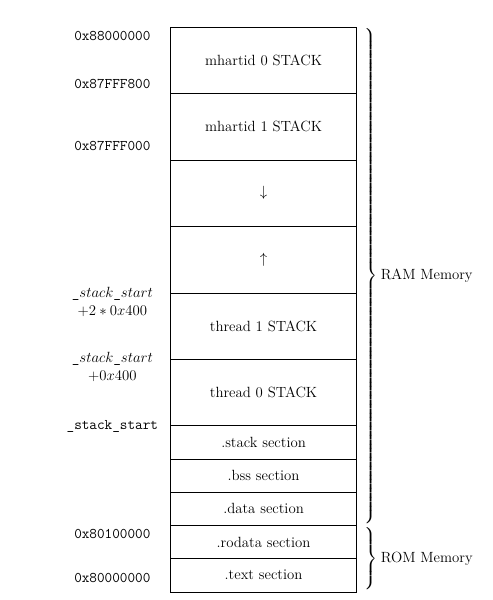
\includegraphics[height=0.65\textheight]{figures/memory.png}
			\end{center}
			\caption{Design of memory layout.}\label{fig:mem_layout1}
		\end{figure}
	\end{minipage}
\end{frame}

\begin{frame}[hoved]
	\frametitle{Implementation}
	\begin{minipage}[t]{0.45\textwidth}
		{\large Partitioning the lists, and creating the threads}
		\begin{itemize}
			\item mhartid 0 is in charge of partitioning the list.
			\item Each thread merges a subsection of the list.
			\item When the number of cores is equal to the number of elements on a
			      level, the context is instead to mergesort that subsection.
			\item Each core can offset into the global THREADS list, for the next
			      element it has to sort.
			\item Using the atomic extension, each core tells parent when they finish.
		\end{itemize}
	\end{minipage}
	\hfill
	\begin{minipage}[t]{0.45\textwidth}
		\begin{figure}
			\begin{center}
				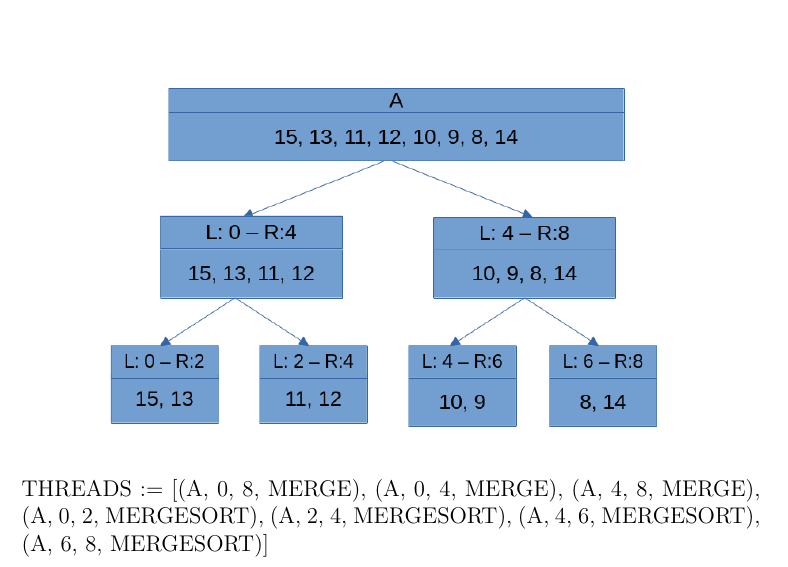
\includegraphics[width=0.95\textwidth]{figures/partitioning.png}
			\end{center}
			\caption{Design of memory layout.}\label{fig:partition}
		\end{figure}
	\end{minipage}
\end{frame}
